\begin{exo}
	Dans un lycée, $60$\% des élèves ont une calculatrice graphique dont $80$\% sont de marque $A$.

	Si la calculatrice n'est pas graphique, alors elle est de marque $A$ dans $50$\% des cas.

	On emprunte la calculatrice d'un élève au hasard et on considère les événements suivants :
	\begin{itemize}
		\item $G$ : \og{} Sa calculatrice est graphique. \fg{}
		\item $A$ : \og{} Sa calculatrice est de marque $A$ \fg{}
	\end{itemize}

	\begin{enumerate}
		\item Modéliser la situation à l'aide d'un arbre pondéré mettant en jeu les événements $G$ et $A$.
		      % \item Quelle est la probabilité que ce soit une calculatrice graphique de marque $A$ ?
	\end{enumerate}
	\begin{center}
		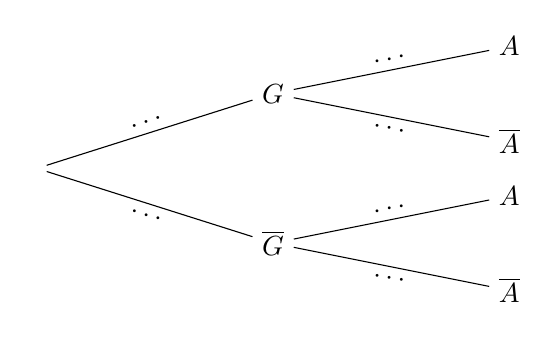
\begin{tikzpicture}[grow=right,sloped, level distance=3cm,
				level 1/.style={sibling distance=1.9cm},
				level 2/.style={sibling distance=1.2cm}]
			\node {}
			child {node {$\overline{G}$}
					child {node {$\overline{A}$} edge from parent node[below] {$\ldots$}}
					child {node {$A$} edge from parent node[above] {$\ldots$}}
					edge from parent node[below] {$\ldots$}
				}
			child {node {$G$}
					child {node {$\overline{A}$} edge from parent node[below] {$\ldots$}}
					child {node {$A$} edge from parent node[above] {$\ldots$}}
					edge from parent node[above] {$\ldots$}
				};
		\end{tikzpicture}
	\end{center}

\end{exo}
